% Options for packages loaded elsewhere
\PassOptionsToPackage{unicode}{hyperref}
\PassOptionsToPackage{hyphens}{url}
%
\documentclass[
  12pt,
  french,
  oneside]{article}
\usepackage{lmodern}
\usepackage{amssymb,amsmath}
\usepackage{ifxetex,ifluatex}
\ifnum 0\ifxetex 1\fi\ifluatex 1\fi=0 % if pdftex
  \usepackage[T1]{fontenc}
  \usepackage[utf8]{inputenc}
  \usepackage{textcomp} % provide euro and other symbols
\else % if luatex or xetex
  \usepackage{unicode-math}
  \defaultfontfeatures{Scale=MatchLowercase}
  \defaultfontfeatures[\rmfamily]{Ligatures=TeX,Scale=1}
  \setmainfont[]{Lato}
\fi
% Use upquote if available, for straight quotes in verbatim environments
\IfFileExists{upquote.sty}{\usepackage{upquote}}{}
\IfFileExists{microtype.sty}{% use microtype if available
  \usepackage[]{microtype}
  \UseMicrotypeSet[protrusion]{basicmath} % disable protrusion for tt fonts
}{}
\makeatletter
\@ifundefined{KOMAClassName}{% if non-KOMA class
  \IfFileExists{parskip.sty}{%
    \usepackage{parskip}
  }{% else
    \setlength{\parindent}{0pt}
    \setlength{\parskip}{6pt plus 2pt minus 1pt}}
}{% if KOMA class
  \KOMAoptions{parskip=half}}
\makeatother
\usepackage{xcolor}
\IfFileExists{xurl.sty}{\usepackage{xurl}}{} % add URL line breaks if available
\IfFileExists{bookmark.sty}{\usepackage{bookmark}}{\usepackage{hyperref}}
\hypersetup{
  pdftitle={Rapport Modélisation en Epidémiologie},
  pdflang={fr-fr},
  pdfkeywords={MEPI, Rennes 1, Projet},
  hidelinks,
  pdfcreator={LaTeX via pandoc}}
\urlstyle{same} % disable monospaced font for URLs
\usepackage[left = 2cm,right = 2cm,top = 2cm,bottom = 2cm]{geometry}
\usepackage{longtable,booktabs}
% Correct order of tables after \paragraph or \subparagraph
\usepackage{etoolbox}
\makeatletter
\patchcmd\longtable{\par}{\if@noskipsec\mbox{}\fi\par}{}{}
\makeatother
% Allow footnotes in longtable head/foot
\IfFileExists{footnotehyper.sty}{\usepackage{footnotehyper}}{\usepackage{footnote}}
\makesavenoteenv{longtable}
\usepackage{graphicx,grffile}
\makeatletter
\def\maxwidth{\ifdim\Gin@nat@width>\linewidth\linewidth\else\Gin@nat@width\fi}
\def\maxheight{\ifdim\Gin@nat@height>\textheight\textheight\else\Gin@nat@height\fi}
\makeatother
% Scale images if necessary, so that they will not overflow the page
% margins by default, and it is still possible to overwrite the defaults
% using explicit options in \includegraphics[width, height, ...]{}
\setkeys{Gin}{width=\maxwidth,height=\maxheight,keepaspectratio}
% Set default figure placement to htbp
\makeatletter
\def\fps@figure{htbp}
\makeatother
\setlength{\emergencystretch}{3em} % prevent overfull lines
\providecommand{\tightlist}{%
  \setlength{\itemsep}{0pt}\setlength{\parskip}{0pt}}
\setcounter{secnumdepth}{-\maxdimen} % remove section numbering
\ifxetex
  % Load polyglossia as late as possible: uses bidi with RTL langages (e.g. Hebrew, Arabic)
  \usepackage{polyglossia}
  \setmainlanguage[]{french}
\else
  \usepackage[shorthands=off,main=french]{babel}
\fi

\title{Rapport Modélisation en Epidémiologie}
\date{}

\begin{document}
\maketitle

\hypertarget{objectif-du-moduxe8le}{%
\section{Objectif du modèle}\label{objectif-du-moduxe8le}}

L'objectif de ce modèle est d'observer la dynamique de la transmission
de la dengue par le moustique \emph{Aedes albopictus}. Cette maladie
infectieuse menace chaque année près de 40\% de la population mondiale
et infecte chaque année entre 50 et 100 milions de personnes selon
l'OMS. L'originalité de ce modèle est qu'il ne s'intéresse pas à la
principale espèce de moustique vecteur de la dingue qui est \emph{Aedes
aegypti}. Si les auteurs préfères s'intéresser à \emph{Aedes
albopictus}, c'est parce que cette espèce a été la cause de plusieurs
épidémie de dengue, cette espèce est plus difficile à contrôler, elle a
un taux de morsure supérieur et est plus compétitivz qu'\emph{A.
aegypti}.

Les auteurs ont créé un premier modèle en couplant un modèle classique
SEIR pour modéliser la dynamique de l'infection chez l'Homme avec un
modèle SEI pour modéliser la dynamique de la maladie chez le vecteur.

Le modèle de dynamique chez l'Homme est le suivant :

\begin{equation} \frac{dH_s}{dt} = \lambda H_t - H_s \left(\frac{cV_i}{H_t} + \mu_h\right)\label{eq:eq1}\end{equation}
\begin{equation} \frac{dH_e}{dt} = H_s \frac{cV_i}{H_t} - H_e (\tau_{exh} + \mu_h)\label{eq:eq2}\end{equation}
\begin{equation} \frac{dH_i}{dt} = H_e\tau_{exh} - H_i\left(\tau_{ih} + \alpha + \mu_h\right)\label{eq:eq3}\end{equation}
\begin{equation} \frac{dH_r}{dt} = H_i\left(\tau_{ih}\right) - \mu_h H_r\label{eq:eq4}\end{equation}

Avec les équations \ref{eq:eq1}, \ref{eq:eq2}, \ref{eq:eq3},
\ref{eq:eq4} faisant référence respectivement au nombre de personnes
sensisbles, exposées, infectées, immunisées. Le modèle de dynamique
épidémiologique pour le moustique est celui-ci :

\begin{equation} \frac{dV_s}{dt} = \mu_aV_t - V_s \left(\frac{cH_i}{H_t} + mu_a\right)\label{eq:eq5}\end{equation}
\begin{equation} \frac{dV_e}{dt} = V_s \frac{cH_i}{H_t} - V_e \left(\tau_{ex\nu} + \mu_a\right)\label{eq:eq6}\end{equation}
\begin{equation} \frac{dV_i}{dt} = V_e\tau_{ex\nu} - \mu_aV_i \label{eq:eq7}\end{equation}

Les équations \ref{eq:eq5}, \ref{eq:eq6}, \ref{eq:eq7} font quant à elle
références respectivement aux moustiques sensibles, exposés et infectés.

Les paramètres de ce modèle sont présentés dans le tableau \ref{tbl:1}
adapté de Erickson et al. (2010).

\begin{longtable}[]{@{}lcc@{}}
\caption{Paramètres utilisés pour construitre le modèle 1.
\label{tbl:1}}\tabularnewline
\toprule
Nom de la variable & Variable & Valeur\tabularnewline
\midrule
\endfirsthead
\toprule
Nom de la variable & Variable & Valeur\tabularnewline
\midrule
\endhead
Taux de croissance de la population humaine & \(\lambda\) &
\(5,8\times 10^{-5}\)\tabularnewline
Taux de mortalité humaine & \(\mu_h\) & \(1/28000\) jours\tabularnewline
Pourcentage journalier de vecteur nécessitant un second repas & \(s_f\)
& \(0.03\)\tabularnewline
Probabilité de mordre un humain & \(b_h\) & \(0,3\)\tabularnewline
Probabilité de transmettre la dengue & \(t_p\) & \(0,4\)\tabularnewline
Probabilité de contact & \(c\) & \(b_h \times t_p\)~\tabularnewline
Inverse du temps d'exposition de l'hôte & \(\tau_{exh}\) & \(1/10\)
jours\tabularnewline
Taux de mortalité des hôtes de la dengue & ~ \(\alpha\) &
\(0,003\)\tabularnewline
Inverse du temps d'infection de l'hôte & \(\tau_{ih}\) & ~ \(1/4\)
jours\tabularnewline
Oeufs par ponte & \(e_p\) & \(30\)\tabularnewline
Inverse du temps de développement des oeufs & \(\tau_e\) &
\(0,361\)\tabularnewline
Taux de mortalité des oeufs & ~\(\mu_e\) & ~\(0,05\)\tabularnewline
Terme de capacité de charge & ~ \(K\) & \(10^{-3}\)\tabularnewline
Inverse du temps de développement des larves & ~ \(\tau_l\) &
\(0,134\)\tabularnewline
Taux de mortalité des larves & \(\mu_l\) & \(0.025\)\tabularnewline
Inverse du temps de développement des nymphes & ~ \(\tau_p\) &
\(0,342\)\tabularnewline
Taux de mortalité des nymphes & \(\mu_p\)~ & \(0,0025\)\tabularnewline
Inverse du temps de développement des adultes immaturees & \(\tau_i\) &
\(1\)\tabularnewline
Inverse du temps de développement des adultes immaturees & \(\tau_i\) &
\(1\)\tabularnewline
Taux de mortalité des adultes & ~ \(\mu_a\) & \(0,0501\)\tabularnewline
Inverse du temps d'exposition du vecteur & \(\tau_{ex\nu}\) & \(1/9\)
jours\tabularnewline
Temps de nourissage ou de gestation & ~ \(\tau_g\) &
\(0.401\)\tabularnewline
Inverse du temps de reproduction & \(\tau_r\) & \(1\)\tabularnewline
\bottomrule
\end{longtable}

Ce premier modèle relativement simple a été ensuite largement modifié
par les auteurs. Ces derniers ont créé un second modèle en divisant le
cycle de vie du moustique \emph{A. aegypti} en six stades de vie
distincts :

\begin{enumerate}
\def\labelenumi{\arabic{enumi}.}
\tightlist
\item
  Oeufs ;
\item
  Larves ;
\item
  Nymphes ;
\item
  Adultes immatures ;
\item
  Adultes en gestation ;
\item
  Adultes capable de se reproduire.
\end{enumerate}

Seul les deux derniers stades de ce cycle de vie peuvent donner lieu à
l'infection d'un être humain sensible. En effet, les femelles ayant
atteint ces stades de vies doivent consommer du sang pour pouvoir
assurer la survie de leurs oeufs. Ce second modèle a été évalué par les
auteurs à une température constante de 25°C.

Dans un troisième temps, les auteurs de cet article ont modifié ce
troisième modèle pour forcer certaines variables controllant le modèle
2. Les variables influencées par la température sont :

\begin{itemize}
\tightlist
\item
  Le temps de développement des oeufs ;
\item
  Le temps de développement des larves ;
\item
  Le temps de gestation des oeufs ;
\item
  Le taux de mortalité des adultes.
\end{itemize}

Pour réaliser ces trois modèles, auteurs de cet articles se basent sur
quatre hypothèses :

\begin{itemize}
\tightlist
\item
  La population à une exposition homogène aux moustiques ;
\item
  Il n'y a pas de migration humaine ;
\item
  Il n'y a pas de migration de vecteur ;
\item
  Il existe qu'un seul serotype de la dengue.
\end{itemize}

L'hypothèse la plus contraignante pour le modèle est la dernière. Il
existe en réalité plusieurs sérotypes pour ce virus. Hors, si une
personne a déjà été infectée par le passé elle devrait se trouver dans
le compartiment immunisés et non pas succeptible. De plus, une personne
déjà infectée par un serotype peut être infectée par un autre serotype.
Si cette hypothèse était relaxée, elle complefirai grandement les
équations consernant les compartiments succeptibles et immunisés.

\hypertarget{reproductibilituxe9-de-larticle}{%
\section{Reproductibilité de
l'article}\label{reproductibilituxe9-de-larticle}}

Pour ce projet, nous avons essayé de reproduire les principaux résultats
de cet article à savoir les principaux graphiques de ce modèle. Le
premier modèle a été relativement simple à coder en R, puisque le nombre
d'équation est relativement restraint.

C'est en essayant de coder par nous-même ce modèle que nous avons
rencontrer les points négatifs de cet article : la reproductibilité.
Bien que les équations soient relativement simple dans le premier
modèle, il existe déjà des erreurs de mise en page concernant les
équations. Ces erreurs ont été facilement contourné grâce aux autres
modèles de l'article qui ne sont qu'une extension du premier. Néanmoins,
corriger ces premières erreurs n'a pas été suffisant pour faire
fonctionner ce premier modèle : il y avait d'autres erreurs plus
incidieuses.

Le tableau décrivant les valeurs des différents paramètres contient lui
aussi des erreurs de mise en page. Le premier modèle ne contenait qu'une
seule erreur dans les paramètres, mais la trouver nous a pris plusieurs
heures. La correction quant à elle était simple à mettre en place.
Finalement, nous avons réussi à recréer les résultats pour ce premier
modèle \ref{fig:model1}.

\begin{figure}
\hypertarget{fig:model1}{%
\centering
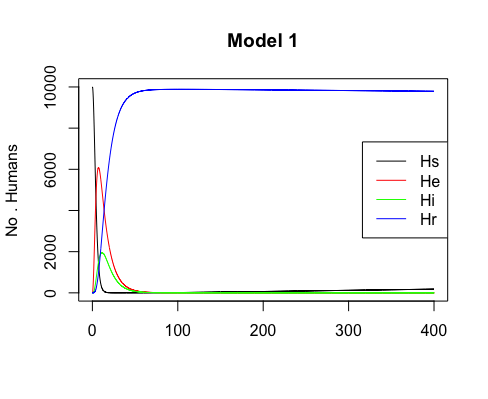
\includegraphics{figures/Model1.png}
\caption{Reproduction de la figure 3c de l'article.}\label{fig:model1}
}
\end{figure}

Pour les modèles 2 nous n'avons pas réussi à reproduire les résultats
des auteurs, car nous avons décelés dans les équations pas moins de 6
fautes différentes. Nous avons essayer de les corriger au mieux, mais
nos résultats ne convergent pas vers ceux trouver par les auteurs
\ref{fig:model2}.

\begin{figure}
\hypertarget{fig:model2}{%
\centering
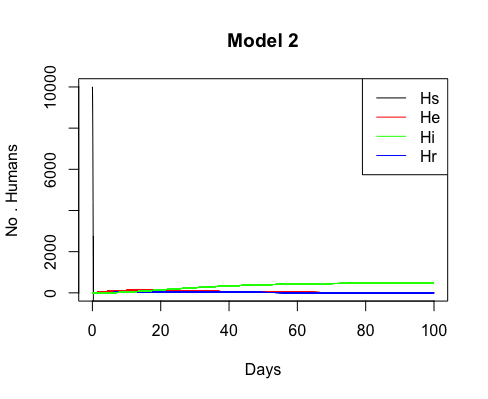
\includegraphics{figures/Model2.png}
\caption{Résultat du modèle 2}\label{fig:model2}
}
\end{figure}

Il est possible que nos corrections soient également érronées, ou bien
alors qu'il y ait d'autres erreurs dans les paramètres du modèles.
Certains paramètres sont des fonctions dépendants de la température, or
l'article ne contient pas ces fonctions mathématiques. L'article
contient uniquement leurs images pour une température de 25°C. Nous
supposons qu'il y a également des erreurs de typographie pour les images
de ces fonctions. Pour les paramètres consernés, nous avons essayé de
nombreuses autres valeurs, mais aucune ne convenait. Les auteurs
indiquent seulement que nous pouvont trouver ces equations dans le
mémoire de master de l'auteur principal. Cependant, aucune version de ce
mémoire n'est disponible en ligne.

Pour le dernier modèle, même s'il nous avait été possible de faire
fonctionner le deuxième modèle, nous n'aurrions pas pu le reproduire. En
effet, les auteurs de cet article expliquent avoir fait varier la
température grâce à la températures de l'air moyenne de la ville de
Lubbock au Texas. Bien que ces données soient disponible sur internet,
le fait de ne pas avoir accès aux fonctions mathématiques dont les
images servent de paramètres aux modèles 2 et 3 nous empêche de les
reproduire.

\hypertarget{moduxe9lisation-compluxe9mentaire}{%
\section{Modélisation
complémentaire}\label{moduxe9lisation-compluxe9mentaire}}

Pellentesque ac porta purus. Phasellus et pellentesque lacus, pulvinar
vulputate dui. Pellentesque posuere pellentesque nisi vel ultricies.
Vivamus at neque convallis, dignissim magna eget, aliquet ante. Maecenas
venenatis, diam in maximus varius, felis ligula faucibus tellus, at
tincidunt ligula ex eu mi. Nunc volutpat leo a nunc laoreet commodo. In
hac habitasse platea dictumst. Aenean pellentesque arcu ut lacus
pulvinar semper. Etiam convallis, magna maximus congue gravida, urna leo
porttitor felis, ut luctus turpis lacus in enim. Vestibulum volutpat
nulla libero, id cursus lacus faucibus sed. Quisque finibus metus quis
lorem iaculis, a scelerisque diam tincidunt. Nulla placerat blandit
quam, eu posuere augue. Cras sem ligula, sodales non sem at, interdum
pretium quam. Cras eget justo blandit, lobortis diam sit amet, eleifend
lorem.

\hypertarget{interpruxe9tations}{%
\section{Interprétations}\label{interpruxe9tations}}

Pellentesque bibendum libero metus, sed laoreet nisl ornare eget.
Interdum et malesuada fames ac ante ipsum primis in faucibus. Morbi
varius mauris eu ipsum pellentesque accumsan a vitae turpis. Sed laoreet
finibus purus, venenatis facilisis mi. Curabitur molestie dui nibh, non
condimentum metus efficitur nec. Fusce nisl eros, bibendum et fermentum
vel, commodo eu est. Sed tristique eleifend felis, sed porttitor tellus
luctus non. Mauris eros metus, rhoncus viverra imperdiet eget, tempor in
odio. Aliquam dapibus pharetra tortor sit amet fermentum.

\hypertarget{synthuxe8se}{%
\section{Synthèse}\label{synthuxe8se}}

Proin eleifend eros eget ante porta, at hendrerit urna pharetra. Duis a
lacus condimentum, dignissim lacus et, tincidunt enim. Quisque ac
efficitur velit. Sed semper ligula id lacus venenatis hendrerit.
Phasellus a nisl id sapien porttitor cursus sed sit amet orci. Praesent
blandit feugiat neque ac feugiat. Quisque dictum enim sed velit sodales
pellentesque. In sapien ligula, bibendum ac purus vitae, luctus
venenatis nisl. Nulla nec posuere velit. Suspendisse ex ex, laoreet ac
ante eu, scelerisque tincidunt ipsum. Pellentesque hendrerit vestibulum
mollis. Aliquam et neque hendrerit risus sagittis placerat.

\hypertarget{bibliographie}{%
\section*{Bibliographie}\label{bibliographie}}
\addcontentsline{toc}{section}{Bibliographie}

\hypertarget{refs}{}
\leavevmode\hypertarget{ref-Erickson_2010}{}%
\textbf{Erickson et al.} A dengue model with a dynamic aedes albopictus
vector population. \emph{Ecological Modelling.} Elsevier BV;
221:2899‑908.

\end{document}
